\section{Imperative to Streaming Transformation}
\label{sec:control}

%In a na\"ive approach, we can map each controller in the hierarchy into a VB (\Cref{fig:centralctrl}).
%This strategy suffers from expensive network round-trip delays between the parent and child controllers.
%If the parent controller is an unrolled loop, the parent needs to synchronize with all child controllers, which creates an undesired communication hot spot.
%\Cref{fig:centralctrl}(a) shows an example where synchronization {\em just} between parent and child controllers can produce an incorrect result due to unpredictable network latency.

%The alternative approach explores a different way to execute the expected control schedule correctly. 
%The minimum required synchronization to produce the correct result is to ensure that the computations access the intermediate results in a consistent matter as if the control schedule is strictly enforced. 
%This can be achieved via p2p synchronizations \emph{only} between computations that access a particular shared memory.
%The execution order of computations that access different memories does not need to be enforced, as they do not impact the program outcome.
%Therefore, as long as the computation is executed with the expected number of iterations and the memories are updated consistently, there is no need for any extra synchronization.
%Next, we walk through how \name{} achieves this in more concrete detail.

\subsection{Loop Division}
Between the front-end and the back-end abstractions of \name, an obvious gap is that 
the imperative front-end language can contain arbitrarily nested control hierarchy, whereas
the hardware compute engine can only execute operations that are control-free.
To address this issue, we introduce a new type of loop transformation---loop division---for streaming reconfigurable
accelerators.
Similar to loop fission, loop division breaks a single loop into multiple loops.
The difference is that loop fission generates a sequence of sequentially executed loops, whereas
loop division generates loops executing \emph{concurrently}.
Additionally, loop fission materializes the intermediate results across fissioned loops into arrays,
while loop division use queue to communicate across loops.
Each loop generated from loop division can only execute if all of their input queues are not empty.
\Cref{fig:loopexp1} gives an example of a loop fusion vs. loop division.

\begin{figure*}
\centering
\begin{subfigure}[b]{0.28\textwidth}
\inputminted{python}{code/loopexp1.py}
\caption{Input program}
\end{subfigure}
\hfill
\begin{subfigure}[b]{0.31\textwidth}
\inputminted{python}{code/loopexp1fission.py}
\caption{Loop Fission}
\end{subfigure}
\hfill
\begin{subfigure}[b]{0.32\textwidth}
\inputminted{python}{code/loopexp1division.py}
\caption{Loop Division}
\end{subfigure}
\caption[Example of loop fission vs. loop division]{
  (b) and (c) shows the output of loop fission and loop division of the input program (a), respectively.
  In (b), the first loop is executed entirely before executing the second loop. The intermediate
  result \texttt{tmp} is materialized into an array with the same size as the loop range.
  In (b), the two loops can execute concurrently. The intermediate result is materialized into a
  queue. For each iteration, a loop can execute only if all of its queues are non-empty.
  The second loop can execute as soon as \texttt{tmp} receives the first element.
}
\label{fig:loopexp1}
\end{figure*}

When executing loop division on a single-threaded CPU, the CPU must context switching between the
concurrent loops
and executing the one with cleared input dependencies.
Like loop fission, loop division is likely worsening the performance on a processor architecture, as
the worst-case memory footprint of the intermediate result \texttt{tmp} increases from $O(1)$ to $O(N)$.
On RDAs, the divided loops are executing
concurrently in a streaming pipelined fashion. The size of the \texttt{tmp} can be limit to a small fixed
size, efficiently implemented with a hardware FIFO. 
Although loop transformations are generally optimizations on CPUs,
loop division is a required transformation to converts an infeasible program to a feasible one for Plasticine.

Loop fission is not always safe, as it may alter the execution order of the program.
Loop division, on the other hand, does not change the underlying data-dependency and is always safe.
To achieve this, loop division needs to introduce additional dummy data dependencies across divided
loops to enforce the correct execution order.
\Cref{fig:loopexp2} gives an example of an invalid loop fission and a correct loop division.
\Cref{sec:controlalloc} gives more detail on how \name automatically generates the dummy
data-dependencies to preserve program order.

\begin{figure*}
\centering
\begin{subfigure}[b]{0.28\textwidth}
\inputminted{python}{code/loopexp2.py}
\caption{Input program}
\end{subfigure}
\hfill
\begin{subfigure}[b]{0.32\textwidth}
\inputminted{python}{code/loopexp2fission.py}
\caption{Invalid Loop Fission}
\end{subfigure}
\hfill
\begin{subfigure}[b]{0.31\textwidth}
\inputminted{python}{code/loopexp2division.py}
\caption{Loop Division}
\end{subfigure}
\caption[Example of an illegal loop fission and a legal loop division]{
Example of an illegal loop fission and a legal loop division
}
\label{fig:loopexp2}
\end{figure*}

\subsection{Virtual Context Allocation} 

\begin{figure*}
\centering
\begin{subfigure}[b]{0.4\textwidth}
\inputminted{python}{code/spatialeg.py}
\caption{Pseudo input example}
\label{fig:contexteg}
\inputminted{python}{code/contextalloc.py}
%\missingfigure[figwidth=1\textwidth]{Spatial IR}
\caption{Initial context allocation}
\end{subfigure}
\hfill
\begin{subfigure}[b]{0.5\textwidth}
\inputminted{python}{code/contextsplit.py}
\caption{Request and response division}
\end{subfigure} \\
\vspace{0.2cm}
\begin{subfigure}[b]{0.23\textwidth}
%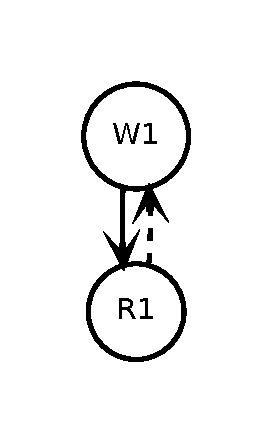
\includegraphics[width=1\textwidth]{figs/dep.pdf}
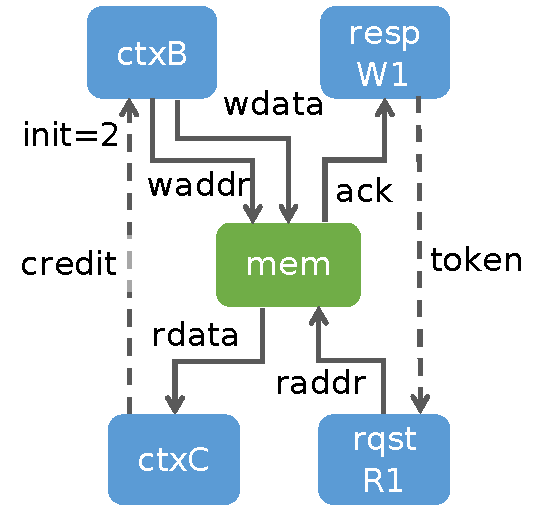
\includegraphics[width=1\textwidth]{figs/ctxdag.pdf}
\caption{Context Graph}
\end{subfigure}
\begin{subfigure}[b]{0.76\textwidth}
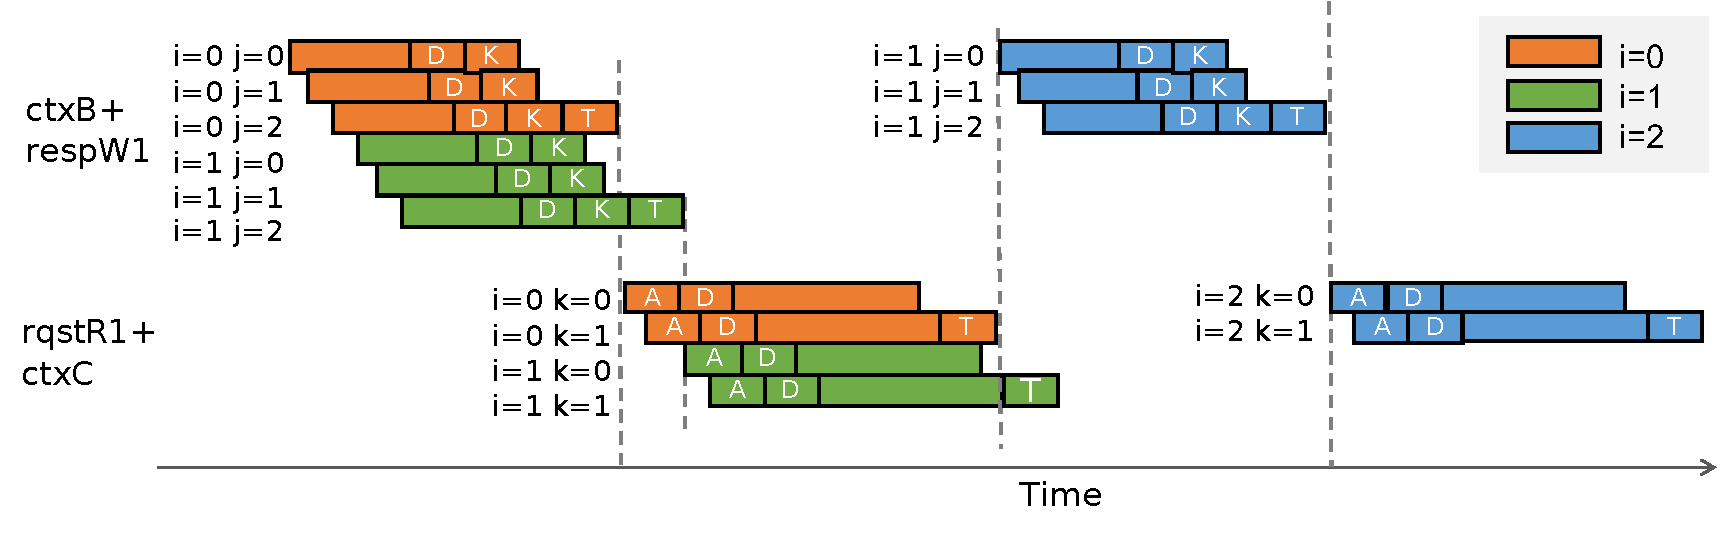
\includegraphics[width=1\textwidth]{figs/plasticinetiming.pdf}
\caption{Timing on Plasticine}
\end{subfigure}
\caption[Context allocation and control allocation]{
  Context lowering and control allocation example.
  %Same example as \Cref{fig:spatialegpar} without outer loop
  %unrolling factor equals to 1.
  %(a) has two basic blocks within the inner most controllers \texttt{B} and \texttt{C}.
  \name allocates one context per basic block for \texttt{B} and \texttt{C}, shown in (b). Outer controller \texttt{A} is
  duplicated in both \texttt{ctxB} and \texttt{ctxC}.
  (c) \name separates out a requesting context \texttt{rqstR1} from \texttt{ctxB} for \texttt{R1} 
  and a receiving context \texttt{respW1} from \texttt{ctxC} for \texttt{W1}.
  The resulting dataflow graph is shown in (d). 
  To enforce the forward data-dependency between \texttt{W1} and \texttt{R1}, 
  \name allocates a forward token between \texttt{W1}'s receiving context \texttt{respW1} and
  \texttt{R1}'s requesting context \texttt{rqstR1};
  to enforce the loop-carried WAR dependency between \texttt{R1} and \texttt{W1}, \name allocates a
  backward token \texttt{credit} between \texttt{R1}'s receiving context \texttt{ctxC} and 
  \texttt{W1}'s requesting context \texttt{ctxB}. 
  The backward token is initialized with two elements because \texttt{mem} is double-buffered,
  enabling the writer for two iterations of A before back-pressured.
  %On the writer side, a forward \texttt{token} is a
  %produced and a backward \texttt{credit} is consumed every \texttt{B} iterations; on the reader
  %side, a forward \texttt{token} is consumed and a backward credit is produced every \texttt{C}
  %iterations. 
  For the forward token, the LCA controller between \emph{W1} and \emph{R1} is \emph{A}. The
  immediate child of the LCA controller in ancestor controllers of \emph{W1} is \emph{B}, therefore,
  the enqueue enable of the token is configured to \emph{B.done} in \emph{respW1}. Similarly on the
  receiving cide, the dequeue enable of the token is \emph{C.done} in \emph{rqstR1}.
  The resulting timing of the execution is shown in (e).
}
\label{fig:contextalloc}
\end{figure*}

\begin{figure*}
\centering
\begin{subfigure}[b]{0.5\textwidth}
  \centering
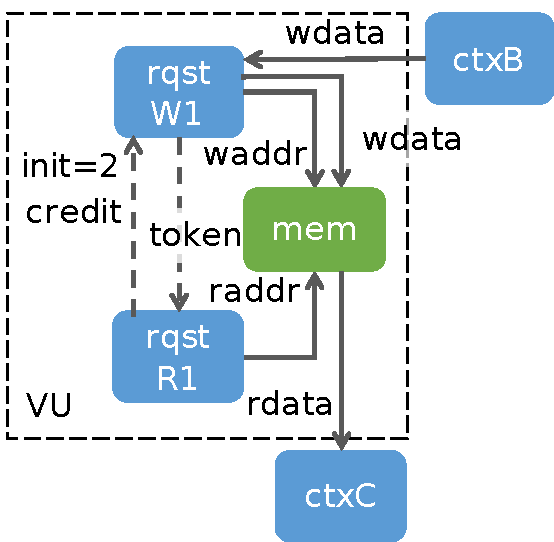
\includegraphics[width=0.6\textwidth]{figs/densespecial.pdf}
\caption{Context dataflow graph}
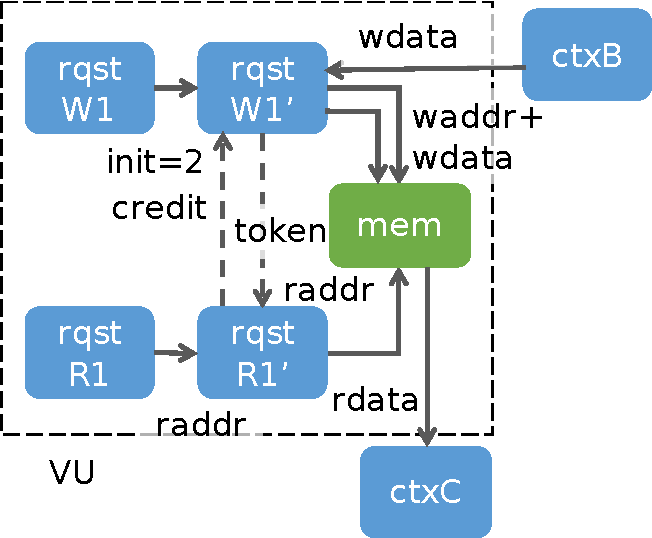
\includegraphics[width=0.7\textwidth]{figs/denseaddr.pdf}
\caption{Optimization for long address calculation}
\label{fig:densespecial}
\end{subfigure}
\hfill
\begin{subfigure}[b]{0.48\textwidth}
  \centering
\inputminted{python}{code/densectx.py}
\caption{Dense specialization}
\end{subfigure} \\
\vspace{0.2cm}
\begin{subfigure}[b]{1\textwidth}
  \centering
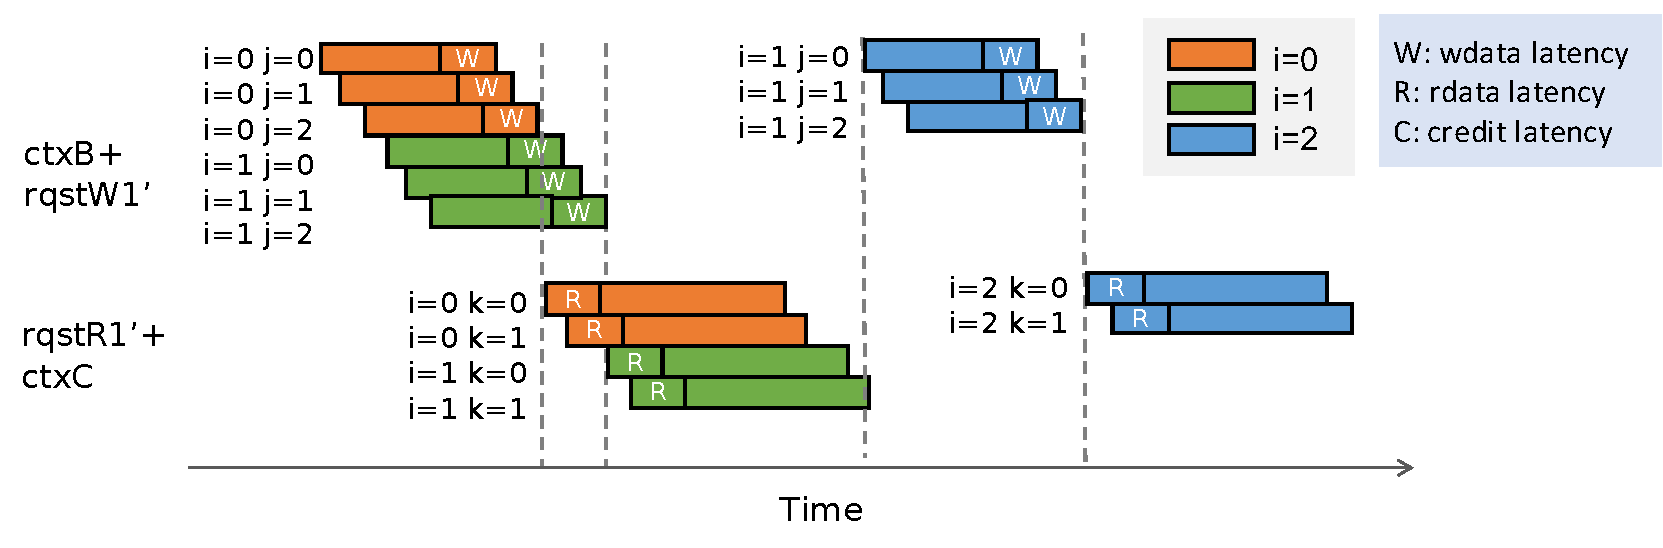
\includegraphics[width=0.85\textwidth]{figs/densetiming.pdf}
\caption{Timing on Plasticine for dense on-chip memory}
\end{subfigure}
\caption[Dense specialization]{
  Specialization for dense memory lowering.
  The same example as \Cref{fig:contextalloc} (a) if the memory is a dense scratchpad.
  (a) and (b) shows the allocated contexts.
  Context \emph{rqstW1} and \emph{rqstR1} are allocated \emph{in the same} VU as the memory. The latency of 
  the forward token and the backward credit take only one cycle, which are not shown in (d).
  The latency to compute read and write addresses are also not shown.
  For complex address calculation, \name split the address computations to separate contexts shown
  in (c). The addresses can be precomputed without waiting for \emph{wdata} for $rqstW1$ and 
  \emph{token} for $rqstR1$.
}
\label{fig:densespecial}
\end{figure*}

At high-level, \name executes the entire program in a pipelined fashion, where each basic block
in the program is a pipeline stage.
As a start, \name allocates a virtual memory to hold each data-structures, and 
a context to execute each basic block within the innermost controllers. 
A basic block maps naturally to a context, as instructions within a basic block are control-free. 
\name makes a copy of all controllers enclosing the basic block in the corresponding context;
these controllers are later converted to counters and control configurations supported by the
hardware. 
Effectively, \name performs loop division such that all basic blocks are perfectly nested.
Contexts are concurrent workers producing and consuming the intermediate data-structures across basic
blocks.

With these controllers, each context can repeatedly execute their basic blocks for an expected number iterations. 
However, data-structures written and read by different contexts are still accessed in random order.
Next, for each virtual memory corresponding to a data-structure, \name examines all contexts accessing the memory,
allocating synchronization tokens across these contexts.
The control token can be viewed as an access grant to the intermediate memory passing between 
the pipelined contexts; the token guarantees the access order of the concurrent contexts is consistent to
the expected order of an imperative program.
The insight is that \emph{as long as all memories are accessed with a program-consistent
order, the final result is identical to a sequentially executed program}.
This way, \name introduces minimum point-to-point synchronizations among small groups of contexts; contexts
accessing different data-structures are naturally parallelized without impacting the final output.
\Cref{fig:contextalloc} (b) shows an example of the context allocation. 
\Cref{sec:controlalloc} explains how \name allocates the synchronization tokens based on the control
hierarchy of the imperative program.

Unlike traditional out-of-order execution, where both static scheduling in the software and dynamic
scheduling in the hardware search for independent instructions to execute concurrently, 
\name starts with executing \emph{all} basic blocks of a program concurrently,
introducing minimum synchronizations wherever necessary.
Unsurprisingly, a control-heavy program with lots of basic blocks can easily run out of PUs.
Nonetheless, the intended workloads for RDAs are data-analytical programs with relatively simple
control flows and abundant data-level parallelism (i.e., most basic blocks having a high repetition
count).
The control flows, however, might not be simple enough that a SIMT architecture, designed for
massive embarrassingly parallel workloads, can still be heavily underutilized.
To map a large program on Plasticine, the program graph must be sliced into multiple chunks.
A single chunk is executed in-space, exploring on-chip parallelism and pipelining;
different chunks are executed in-time by reconfiguring the accelerator.

\subsection{Control Allocation} \label{sec:controlalloc}
\label{sec:sync}
\name uses control tokens to enforce the memory access order in an imperative program on a dataflow
architecture. 
In this section, we first explain \emph{how} \name uses tokens to enforce the memory access 
order between distributed contexts and achieves complex control flows on a data-flow architecture;
next, we show \emph{where} \name inserts these tokens and how to minimize inserted tokens while
enforcing the program order.

%This section answers three essential questions for this transformation: 
%\emph{how} to use tokens to enforce the memory access order between two distributed contexts;
%\emph{when} do contexts send the tokens at runtime;
%and \emph{where} do tokens have to be inserted.
%Starting with all contexts execute in parallel, \name introduces \term{control token}s across contexts
%to serialize their execution order based on the program order.
%This control token is no different from a regular data-dependency and can be viewed as 
%an access grant to the shared memory across contexts. 
%By controlling {\em where}, {\em how}, and {\em when} to pass the token, \name can maintain a consistent update ordering between the pipelined and parallelized contexts that access the shared memory.

%We refer to memory access appeared in the input IR as a \emph{declared access}, as supposed to
%memory accesses executed at runtime.
%\texttt{W1} and \texttt{R1} are examples of two declared accesses in \Cref{fig:contexteg}
%In the rest of this section, we will walk through how \name allocates control tokens
%to maintain sequential consistency on Plasticine.

\paragraph{How.} 
The first question is how do we enforce the access order of a memory from two remotely distributed contexts, given the
global network and the memory itself can introduce unpredictable latency.
The memory interface on Plasticine can take a stream of read or write requests, providing a response
packet for each request packet.
Within a single stream, the requests are guaranteed to be served in order. 
Therefore, the read response is a stream of data (not tagged with request address) and the write response is a stream of control tokens without any payload.
To eliminate the round-trip latency, \name divides each memory access in the input IR into a requesting and a receiving context, as shown in \Cref{fig:contextalloc} (c). 
For a read access, \name maps the address generation in a separate requesting context, streaming
addresses to the memory and streaming the data to the receiving context.
Similarly, for a write access, \name allocates a receiving context to accumulate acknowledgments 
for synchronizations.

%We refer to a memory access appeared in the input IR as a \emph{declared access}, as supposed to
%memory accesses executed at runtime.
%\texttt{W1} and \texttt{R1} are examples of two declared accesses in \Cref{fig:contexteg}
To order an access $A$ before an access $B$,
\name allocates a token between the receiving context of access $A$ ($resp_A$) and the requesting context
of access $B$ ($rqst_B$).
This is essential to ensure the memory effect of access $A$ is visible to access $B$, as the memory
might take multiple cycles to serve a request.
For any two accesses enclosed by a loop in the input IR, there could be a loop-carried dependency (LCD) from
the later access in the program order to the earlier access.
When inserting a token for an LCD, the receiver's token buffer is always initialized with at least one token,
enabling the earlier access for the first iteration of the loop. \Cref{fig:contextalloc} (c) shows the
forward and the backward token to enforce two accesses under a loop. The initial element in backward
token breaks the cyclic dependency. 
Borrowing the flow-control
terminology\cite{credit}, we refer to a backward token as a credit.
If the memory is multi-buffered, the credit is initialized with buffer-depth $D$ number of credit, 
enabling the first access to execute $D$ iterations of the enclosed loop before back-pressured.

\name wires up the enqueue/dequeue enable of a token with signals from the duplicated controllers 
in the writer/reader context.
For a token representing the dependency of a queue, the token should be generated/consumed every cycle when the producer/receiver context is active; to achieve this, \name configures the enqueue/dequeue signal
to the \emph{valid} signal of the innermost controller in the requesting/receiving context.
For a token corresponding to a scalar variable or an array, the program expects the producer/consumer
to update/inspect the memory for every iteration of their LCA controller.
\name finds the LCA controller between the writer and the reader contexts of a token,
connecting the \emph{done} signal of LCA's immediate child in the writer/reader context's ancestor controllers to the enqueue/dequeue enable of the token.
\Cref{fig:contextalloc} (c) shows an example of how the enqueue and dequeue signals are configured.

By controlling \emph{when} a token is produced and consumed, \name is able to achieve the complex
and nesting control flows in an imperative program on a dataflow accelerator.
\Cref{sec:datactrl} dives into more complex control constructs with 
data-dependent control flows.

The requesting and receiving contexts pair are general schemes we use on any type of memory with 
multiple cycle access latencies, such as the off-chip DRAM.
In common cases, we can simplify the synchronization logic for certain on-chip memory types.

\subparagraph{Specialization for dense on-chip scratchpad}
Spatial can statically analyze the dense access pattern of on-chip arrays and partitions the memories
to avoid bank conflicts. These memories have a guaranteed single-cycle access latency, 
which simplifies the synchronization.
\name allocates $rqst_A$ and $rqst_B$ contexts \emph{in the same} VB as the accessed memory.
Instead of synchronizing between $resp_A$ and $rqst_B$, \name sends the forward token and the
backward credit between $rqst_A$ and $rqst_B$,
eliminating the need for a receiving context for the write access.
Because memory requests are served in a single cycle, access $A$'s requests would be visible to
access $B$ by the time $rqst_B$ receives the token. Hence, write acknowledgment is no longer needed.
\Cref{fig:densespecial} shows the resulting contexts if \emph{mem} in \Cref{fig:contexteg} is a dense
on-chip array.

\subparagraph{Specialization for non-indexable memory}
For most non-indexable memories like scalar variables and queues in the program, \name directly maps
them to the input buffer of the receiver context if the memory has a single writer and a single
reader.
Non-indexable memory with multiple readers and writers also need synchronization token across
the accessing contexts to enforce a program-consistent accessing order.
%We perform another specialization on non-indexable memories (registers or FIFOs), whose all accesses have no explicit read enables.
%Instead of treating them as shared memories, \name{} duplicates and maps them to local input buffers in all receivers, no longer requiring tokens.
%The sender actor pushes to the network when the token is supposed to be sent, and the receiver dequeues one element from the input buffer when the token is supposed to be consumed.
%This dramatically reduces the synchronization complexity of non-indexable memory in the common case.

\begin{table*}
  \centering
\begin{tabular}{lccc}
  \toprule
 Data structure & Memory type \\ \midrule
  array (fits on-chip) & SRAM \\
  array (does not fit on-chip) & DRAM \\
  scalar variable & register \\
  queue & FIFO \\
 \bottomrule
\end{tabular}
\caption[Mapping between data-structure to hardware memories]{
  Mapping between user declared data-structure to underlying hardware memories. 
  Programmers explicitly specify the desired hardware type inside Spatial. 
  In other languages, this table specifies a mapping between software data-structures 
  and hardware memory types on Plasticine.
}
\label{tab:memtype}
\end{table*}

\paragraph{Where.}
\name can serialize every accesses pair of a memory to enforce the program order. However, that
would require $N^2$ tokens for a memory with $N$ accesses ($2N^2$ with LDCs) in the input IR, which can be
unnecessarily expensive.
The second question is how can we minimize the number of inserted token while ensuring a correct execution.
To tackle this problem, \name builds a dependency graph between all accesses of a memory in the input IR; 
the dependency graph is \emph{per data-structure} without unnecessary ordering across different memories.
Next, \name removes edges in the dependency graph, if the removed edge does not relax the ordering
across accesses.
Lastly, for each edge in the reduced dependency graph, \name inserts token between the receiving and
requesting contexts of the source and destination access explained earlier in the \emph{How} section.

\subparagraph{Dependency Graph Construction}
For every access in the IR, \name{} checks on other accesses that occurred earlier in the program order
for a possible forward dependency, and later in the program order for a possible loop-carried dependency (LCD). 
%In the example in \Cref{fig:contexteg}, there is a forward data dependency between \texttt{W1} and
%\texttt{R1}, and a write-after-read LCD between \texttt{R1} and \texttt{W1}. 
\name only inserts an edge between two accesses if they potentially interfere, which is a function of
\begin{outline}
  \1 the type of accesses (read vs. write)
  \1 the type of the memory (e.g. SRAM, DRAM)
  \1 and location of the declared accesses in the control hierarchy.
\end{outline}
\Cref{tab:memtype} lists hardware memories available on reconfigurable architectures and software data-structures providing similar program semantics.
The type of the memory matters because they have different programming interface on the hardware.
\Cref{fig:depeg} shows examples of dependency graphs derived from programs.
types.
%For instance, two DRAM read accesses do not interfere because the DRAM interface permits
%multiple concurrent access streams through multiple DAGs\footnote{All DAGs can access the full DRAM
%address space}. 
%%\gist{mension port virtualization}
%Therefore, from the programmer's perspective, users do not need
%to to serialize the two contexts reading the same DRAM address. 
%Plasticine's SRAMs, on the other hand, have a single read and write port. 
%Programmers must guarantee that a PMU receives read requests from a single context
%at any point in time for correctness.
%\Cref{tab:interferetab} shows the interference relation between different types of memory across
%accesses.

\begin{table*}
  \centering
\begin{tabular}{lcccc}
  \toprule
  Memory type             & DRAM   & SRAM   & FIFO   & Register \\ \midrule
  read-after-read (RAR)   & \xmark & \cmark & \cmark & \xmark \\
  read-after-write (RAW)  & \cmark & \cmark & \cmark & \cmark \\
  write-after-read (WAR)  & \cmark & \cmark & \cmark & \cmark \\
  write-after-write (WAW) & \cmark & \cmark & \cmark & \cmark \\
 \bottomrule
\end{tabular}
\caption[Interferance Table]{
  Interference table for whether two accesses of the same memory needs to be synchronized by the
  software for each memory type.
}
\label{tab:interferetab}
\end{table*}

\begin{figure*}
\centering
\begin{subfigure}[b]{0.34\textwidth}
\inputminted{python}{code/dep1.py}
\caption {
  Example with outer loop parallelization.
}
\end{subfigure}
\hfill
\begin{subfigure}[b]{0.3\textwidth}
  \centering
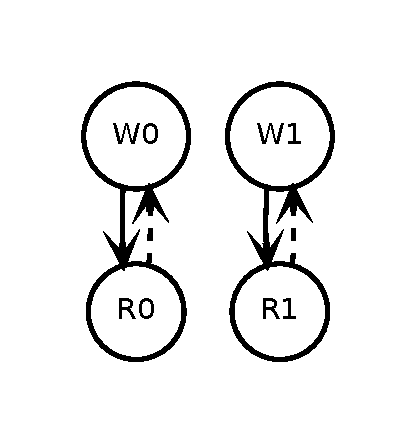
\includegraphics[width=0.6\textwidth]{figs/dep1.pdf}
\caption{
  Access dependency graph for \emph{mem} (on-chip) in (a)
}
\end{subfigure}
\hfill
\begin{subfigure}[b]{0.3\textwidth}
  \centering
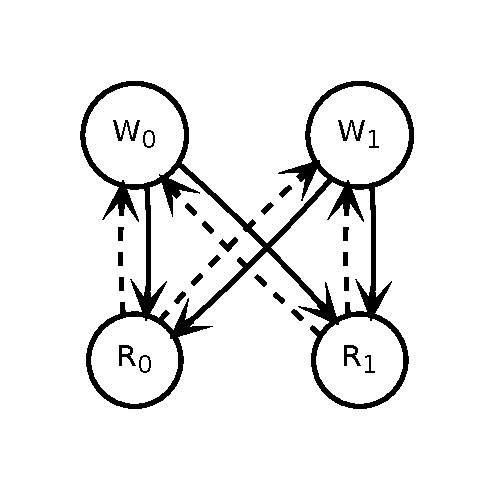
\includegraphics[width=0.7\textwidth]{figs/dep2.pdf}
\caption{
  Access dependency graph for \emph{mem} (off-chip) in (a)
}
\end{subfigure}
\\
\begin{subfigure}[b]{0.4\textwidth}
\inputminted{python}{code/dep3.py}
\caption{Example with branches}
\end{subfigure}
\begin{subfigure}[b]{0.5\textwidth}
  \centering
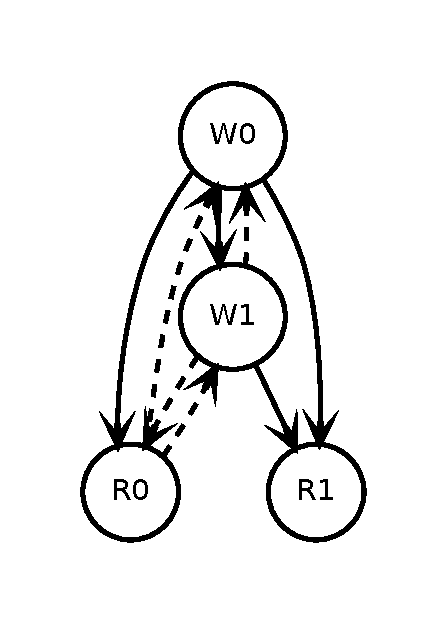
\includegraphics[width=0.4\textwidth]{figs/dep3.pdf}
  \caption{Access dependency graph for \emph{mem} (off-chip) in (d)}
\end{subfigure}

\caption[Examples for access dependency graph]{
  Access dependency graphs for example programs. 
  Solid edges indicate forward dependencies and
  dashed edges indicate backward loop-carried dependencies (LCDs).
  In (b) and (c),
  \emph{$W_0$} and \emph{$W_1$} are unrolled accesses for $W$ in lane 0 and 1 of loop \emph{A}
  in (a), respectively.
  (b) is the dependency graph if the memory is mapped to an on-chip memory and (d)
  is the dependency graph if the memory is mapped to an off-chip memory.
  The on-chip version does not need the cross-lane synchronization because 
  lane 0 and 1 are implicitly ordered when \name partitions \emph{mem} 
  (discussed later in \Cref{sec:memsplit}).
  In (d), there is no forward dependency between \emph{W1} and \emph{R0} because the LCA controller of the two accesses is branch \emph{C}, which means the two accesses cannot happen concurrently in
  the same iteration of \emph{A}.
  There is, however, loop-carried dependencies between \emph{R0} and \emph{W1}. 
  Loop-carried
  dependency on the same access (such as between \emph{R0} and itself across iterations of loop \emph{A}) does not need to be enforced as the streaming memory interface preserves ordering
  within a single requesting stream from the same access.
  For each iteration of \emph{A}, \emph{R0} and \emph{W1} will produce and consume a credit from
  each other no matter what value the condition takes. 
  \Cref{sec:datactrl} will elaborate more on branches.
  \emph{R0} and \emph{R1} do not depend on each other because they are both DRAM read accesses.
}
\label{fig:depeg}
\end{figure*}

\subparagraph{Dependency graph reduction}

\begin{figure*}
\centering
\begin{subfigure}[b]{0.34\textwidth}
\inputminted{python}{code/graphred1.py}
\caption {
  Example program with off-chip \emph{mem}
}
\end{subfigure}
\begin{subfigure}[b]{0.3\textwidth}
  \centering
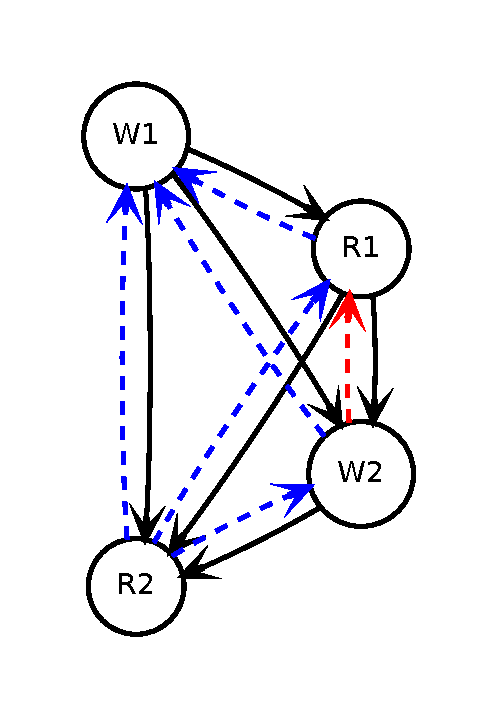
\includegraphics[width=0.6\textwidth]{figs/graphred1.pdf}
\caption{
  Dependency graph before reduction for (a)
}
\end{subfigure}
\begin{subfigure}[b]{0.3\textwidth}
  \centering
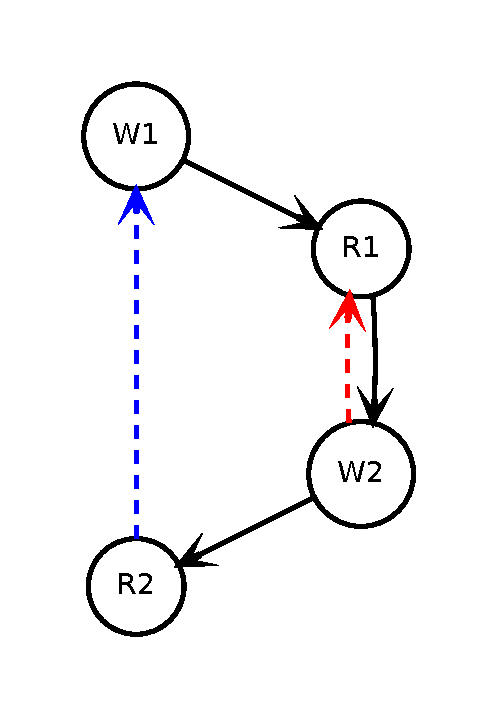
\includegraphics[width=0.6\textwidth]{figs/graphred1_after.pdf}
\caption{
  Dependency graph after reduction for (a)
}
\end{subfigure}
\\
\begin{subfigure}[b]{0.34\textwidth}
\inputminted{python}{code/graphred2.py}
\caption{
  Example program with off-chip \emph{mem}
}
\end{subfigure}
\begin{subfigure}[b]{0.3\textwidth}
  \centering
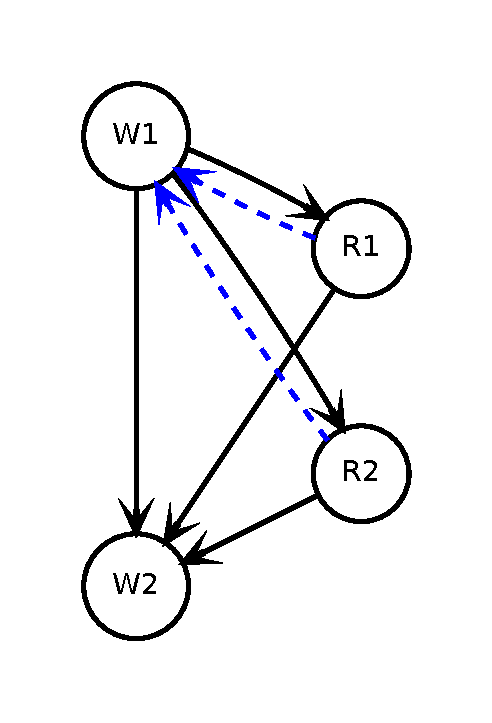
\includegraphics[width=0.6\textwidth]{figs/graphred2.pdf}
\caption{
  Dependency graph before reduction for (d)
}
\end{subfigure}
\begin{subfigure}[b]{0.3\textwidth}
  \centering
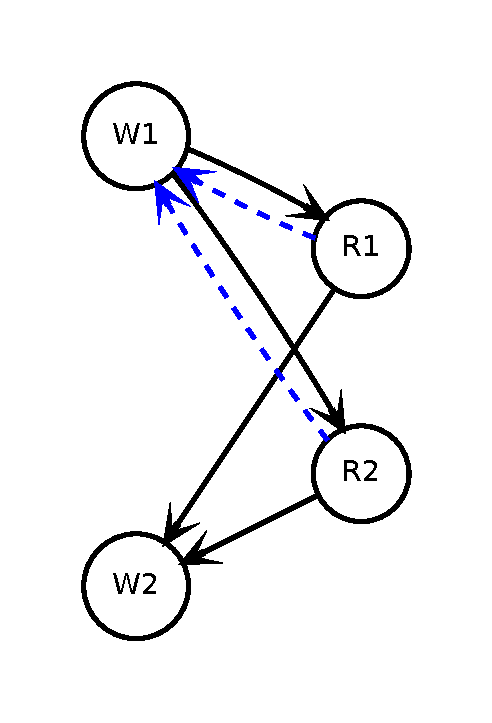
\includegraphics[width=0.6\textwidth]{figs/graphred2_after.pdf}
\caption{
  Dependency graph after reduction for (d)
}
\end{subfigure}
\definecolor{pureblue}{rgb}{0, 0, 255}
\caption[Examples for dependency graph reduction]{
  Dependency graphs (b,e) and reduced dependency graph (c,f) of the example programs (a,d).
  Solid edges indicate forward dependencies and
  dashed edges indicate backward loop-carried dependencies (LCDs).
  Colors of the LCD edges indicate the associated loop, \textcolor{pureblue}{blue} for loop \emph{A} and
  \textcolor{red}{red} for loop \emph{B}.
  For the forward edges (black edges), \name uses transitive reduction to remove the redundant
  edges.
  For the backward edge, an edge can be removed if there is still a path from its source to
  destination with all forward edges plus \emph{a single} backward edge with the same loop after the edge is
  removed.
  For example in (c), edge \emph{R2-R1} is removed because there is path \emph{R2-W1-R1}.
  Edge \emph{W2-W1} is removed because there is path \emph{W2-R2-W1}. 
  Edge \emph{R2-W1} cannot be removed because there is no path from \emph{R2} to \emph{W1} with a
  single back edge after the edge is removed.
  \emph{R2-W1} cannot be
  removed in (e) because there is no path from \emph{R2} to \emph{W1} after the edge is removed.
}
\label{fig:graphred}
\end{figure*}

%Enforcing all dependencies in the dependency graph may not be necessary, as enforcing a subset of
%dependencies can be sufficient to enforce the order of the whole graph.
\name reduces the dependency edges in two passes, processing edges for the forward and backward dependencies separately.

For forward dependencies, \name performs a transitive reduction (TR)\cite{tr} on the forward dependency
graph. TR keeps the minimum of edges in a graph that preserves the connectivity of the original
graph, enforcing the same ordering as the original dependency graph.

Next, \name checks if each backward edge can be removed without breaking the execution order between
accesses. 
Each backward edge represents a loop-carried dependency (LCD) and is tagged with the associated loop.
A backward edge can be removed if after removing the edge, there is a path from the source to the
destination node of the edge; the path may contain any forward edges remained from the TR pass,
with \emph{a single} backward edge tagged with the same loop as the removed edge.
\Cref{fig:graphred} shows examples of dependency graph reduction.

The forward edges can be reduced with TR because the forward dependencies
are monotonic, i.e. \emph{A} depends on \emph{B} and \emph{B} depends on \emph{C}
enforces \emph{A} depends \emph{C}. The backward edges are non-monotonic because of the initial
tokens in the destination buffers.

%\begin{figure*}
%\centering
%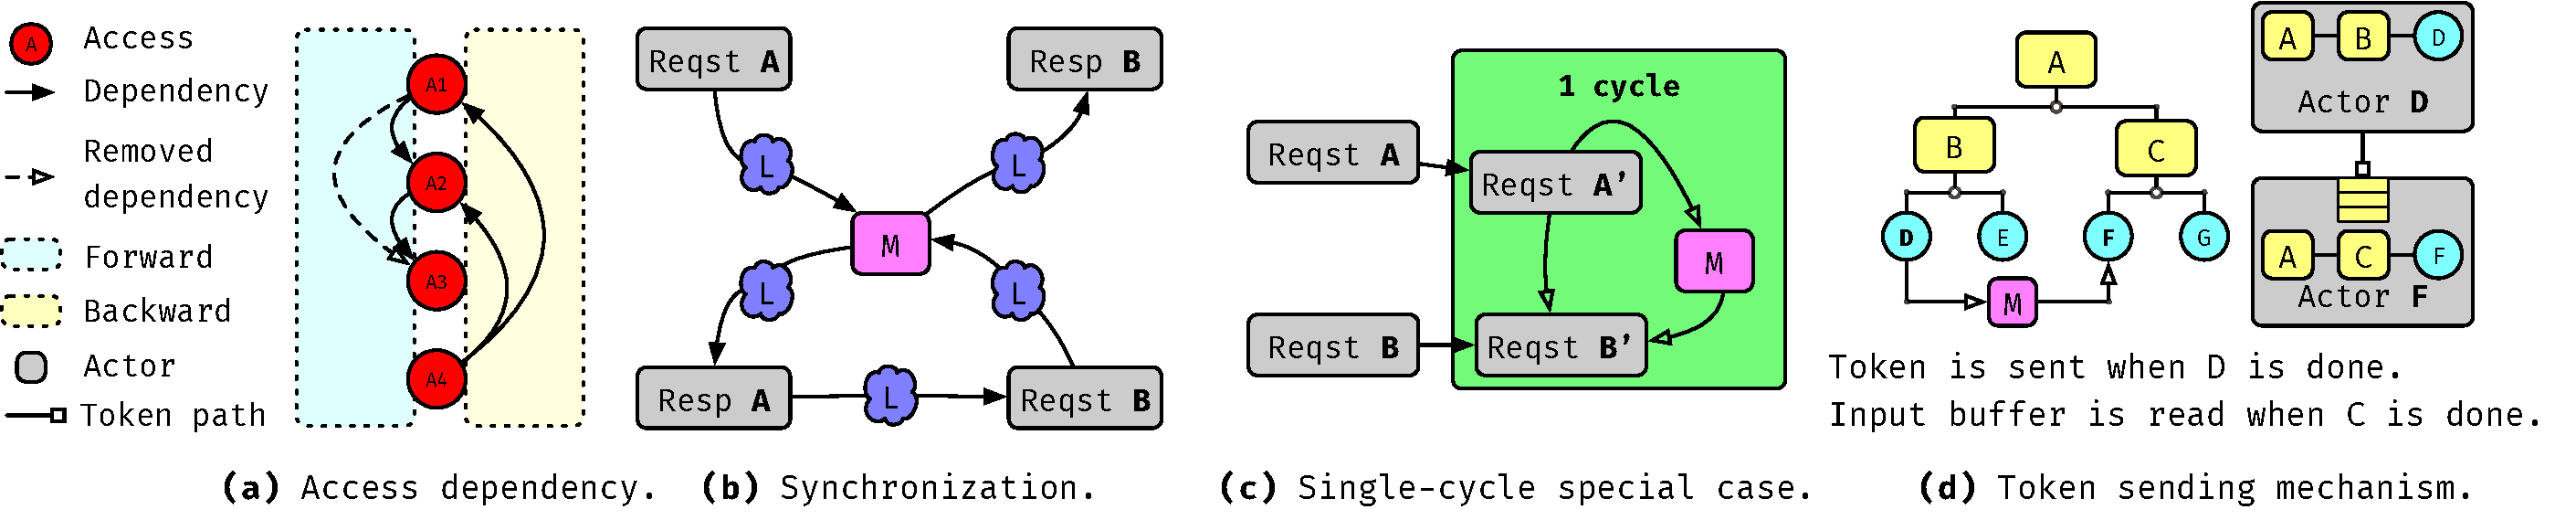
\includegraphics[width=1.0\textwidth]{figs/synch_mech.pdf}
%\caption{
    %(a) Access dependency graph.
    %(b) Synchronization of two accesses on the same memory.
    %(c) Single-cycle special case.
    %(d) Actors uses local states of controller hierarchy to determine when to send a token.
%}\label{fig:depgraph}\label{fig:token}\label{fig:tokentrick}\label{fig:tokenwhen}
%\end{figure*}
%%\ms{repeated caption, rather give a single caption.}


\subsection{Data-Dependent Control Flow} \label{sec:datactrl}
Using the synchronization discussed in \Cref{sec:sync}, \name can support control constructs that 
typically are not supported on dataflow accelerators, such as branches and while loops.
Most dataflow accelerators do not support control divergence. SIMT architectures, like GPUs,
implement branches with predication and pay the latency penalty of both branch cases.
To enable these flexible control, the control path of the architecture must permit data dependencies.
\Cref{fig:controlarch} details the required changes in the control path to support these features.

\paragraph{Dynamic Loop Range}
\Cref{fig:dynrange} shows an example of loops with data-dependent ranges. 
\name uses a context to compute the loop bounds, which are treated as input dependency to the context 
that maps the loop body.
\begin{figure*}
\centering
\begin{subfigure}[b]{0.4\textwidth}
\inputminted{python}{code/dynrange.py}
\caption{Input program}
\end{subfigure}
\hfill
\begin{subfigure}[b]{0.5\textwidth}
\inputminted{python}{code/dynrangectx.py}
\caption{Context data-flow graph}
\end{subfigure}
\caption[Example of dynamic loop range]{
  (a) shows an example program with dynamic loop range. 
  Expressions to generate the loop bounds belongs to a basic block that gets mapped to \texttt{ctx1}.
  \name maps the loop bound as a data-dependnecy to context that maps the inner loop context, and
  configures dequeue signal of \texttt{bound} stream to counter \texttt{B.done}.
}
\label{fig:dynrange}
\end{figure*}

\begin{figure*}
\centering
  \vspace{-1cm}
\begin{subfigure}[b]{0.45\textwidth}
\inputminted{python}{code/branch.py}
\caption{Input program}
  \vspace{0.2cm}
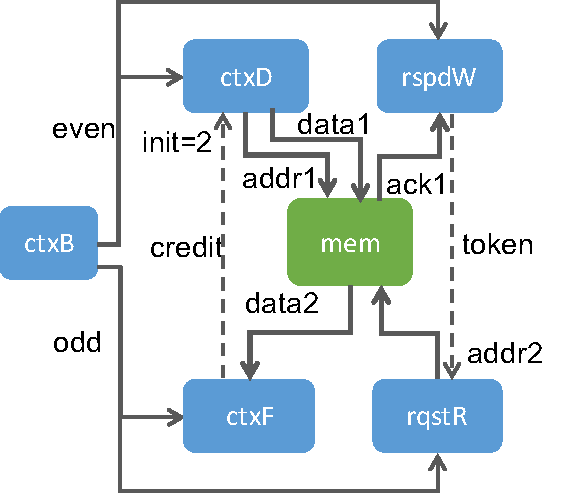
\includegraphics[width=0.8\textwidth]{figs/branchctx.pdf}
\caption{Dataflow graph}
\end{subfigure}
\hfill
\begin{subfigure}[b]{0.48\textwidth}
\inputminted{python}{code/branchctx.py}
\caption{Context configuration}
\end{subfigure}
\\
  \vspace{0.2cm}
\begin{subfigure}[b]{\textwidth}
  \centering
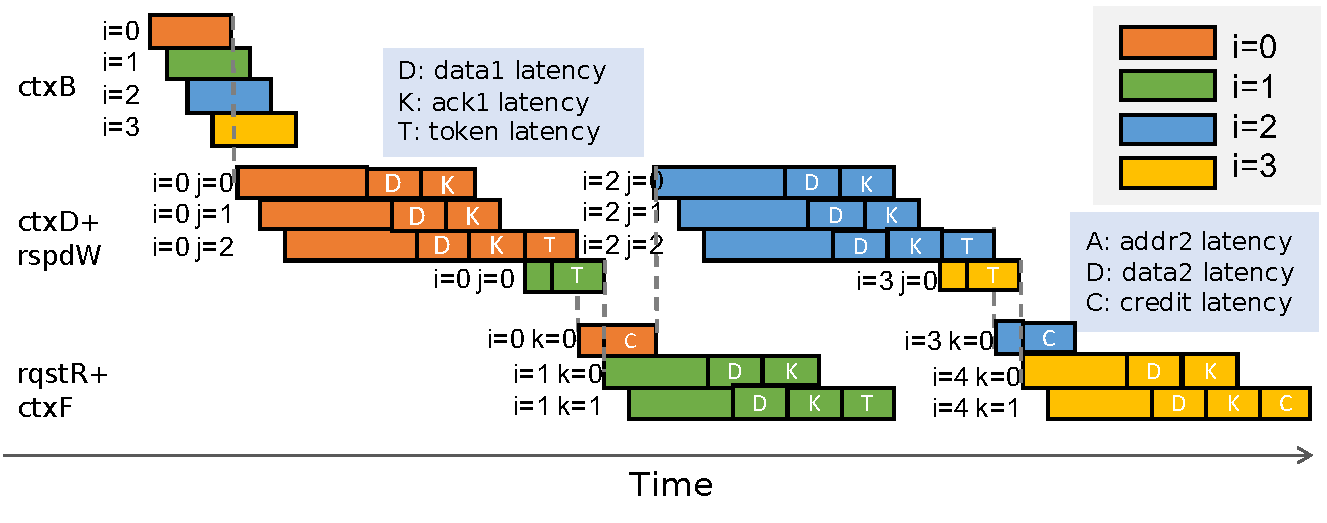
\includegraphics[width=0.8\textwidth]{figs/branchtiming.pdf}
\caption{Timing}
\end{subfigure}
\caption[Branching example]{
  An example program with a branch. 
  (d) shows the timing of execution with $A=4$, $D=3$, and $F=2$.
}
\label{fig:branch} 
\end{figure*}

\paragraph{Branch Condition}
\name supports both predictions and branches with control divergence.
Branches within the innermost loops are implemented with predication such that the loop can still be
vectorized across SIMD lanes.
This is very similar to a SIMT architecture, where all lanes execute the \emph{if} clause followed by the \emph{else} clause, masking off the memory access for the disabled lanes.
The total number of SIMD stages required is the total operations in both the \emph{if} and the \emph{else} clauses.

For a branch in an outer loop,
the branch condition is treated as a data-dependent enable signal for controllers under the branch clauses.
If the controller is disabled, its \emph{done} signal raises to high immediately.
Output tokens depending on the {\em done} signal will be immediately sent out.
This way, the controller under a branch condition does not need to execute if the outer branch
evaluates to false.

\Cref{fig:branch} shows an example with a branch statement.
The input program in (a) writes and reads the memory \emph{mem} on even and odd cycles of
the outer loop \emph{A}, respectively. 
\name maps the three basic blocks in the program in three
contexts, \emph{ctxB}, \emph{ctxD}, and \emph{ctxF}, as shown in (b) and (c). 
For the read and write accesses, \name
allocates a context \emph{respW} to accumulate write acknowledgments and a context \emph{rqstR} 
to generate read requests. 
\emph{ctxB} generates the branch conditions for both the \emph{if} and the \emph{else} clauses.
The conditions are sent as data dependencies to contexts mapping the basic blocks under the branch conditions.

\Cref{fig:branch} (d) shows the timing of execution.
As \emph{ctxB} has no dependencies, \emph{ctxB} computes the conditions for all iterations of
\emph{A} in
pipelined fashion and broadcasts the conditions to the receiver contexts.
The \emph{if} contexts (\emph{ctxD}+\emph{rspdW}) receives a \texttt{true} condition for the first
iteration of \emph{A} ($A_0$), 
executing all iterations of D, and passes a token to the \emph{else} (\emph{rqstR}+\emph{ctxF}) contexts.
Because \emph{mem} is double-buffered, the credit is initialized with two elements in the
receiver's input buffer, enabling the \emph{if} contexts to execute two iterations of outer loop
\emph{A} before
waiting for the \emph{else} contexts. For the second iteration of loop \emph{A} ($A_1$), the \emph{if} contexts
receives a \texttt{false} condition for branch \emph{C}.
Therefore, the enclosing loop controller \emph{D}'s \emph{done} signal is immediately high, sending the
token to \emph{rqstR} context right away.
On the other side, the $A_0$ of the \emph{else} contexts is blocked by the token from
the \emph{if} contexts. 
As soon as the token arrives, the \emph{else} contexts send out the credit immediately,
Next, the \emph{else} contexts check for the second token, 
and executes loop \emph{F} for $A_1$.

Both the \emph{if} and the \emph{else} contexts only execute if their enclosed branch clauses are
evaluated to be true. More interestingly, \Cref{fig:branch} (d) shows a overlapping execution of the
\emph{if} and \emph{else} clauses across iterations of A. 
The hardware for both \emph{if} and \emph{else} clauses are active almost all time.
If the latency of loop \emph{D} and \emph{F} are both $L$, 
the total runtime for $N$ iterations of loop \emph{A} would be on the order of $\frac{N}{2}L+L$
on Plasticine, assuming L and N are large.
\emph{This is almost twice as fast as a traditional coarse-grained pipelining with hierarchical FMS
schedulers}, like Spatial's FPGA back-end, whose runtime is $NL+L$.

\paragraph{Do While Loops}

\begin{figure*}
\centering
  \vspace{-1cm}
\begin{subfigure}[b]{0.45\textwidth}
\inputminted{python}{code/dowhile.py}
\caption{Input program}
  \vspace{0.2cm}
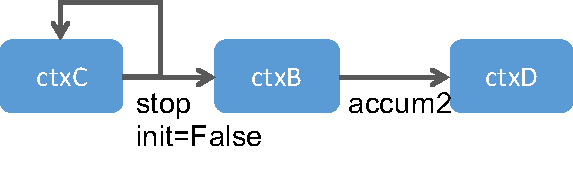
\includegraphics[width=0.8\textwidth]{figs/dowhile.pdf}
\caption{Dataflow graph}
\end{subfigure}
\hfill
\begin{subfigure}[b]{0.48\textwidth}
\inputminted{python}{code/dowhilectx.py}
\caption{Context configuration}
\end{subfigure}
\\
  \vspace{0.2cm}
\begin{subfigure}[b]{\textwidth}
  \centering
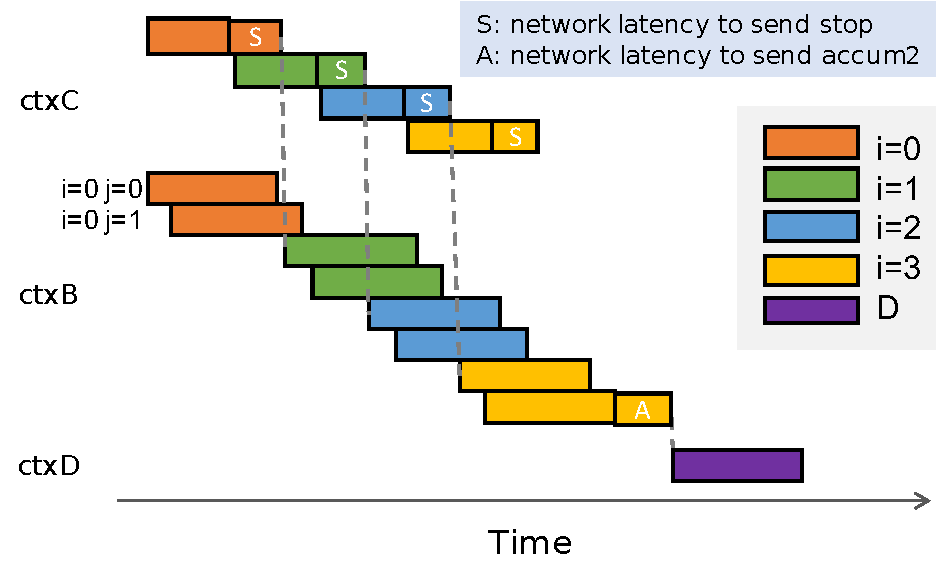
\includegraphics[width=0.6\textwidth]{figs/dowhiletiming.pdf}
\caption{Timing}
\end{subfigure}
\caption[Do while example]{
  An example program for do while loop. 
  Loop \emph{A} in (a) is a loop running forever, with a conditional \emph{stop} variable.
  The break statements in (c) corresponds to configuring the stop signal of the enclosing controller \emph{A}
  to the output of the stop input buffer. The stop buffer is dequeued every cycle controller \emph{A} is active.
}
\label{fig:dowhile} 
\end{figure*}

The \emph{do while} construct is very useful to express iterative convergence algorithms or handle external
data stream with a last-bit signal that terminates the execution.
A \emph{do while} loop works very similarly to a loop with dynamic range, except the loop has a very long
initialization interval. The earliest starting time for the second iteration of the loop is when the while condition is resolved.
The while condition is a data-dependency to all contexts mapping the basic blocks enclosed by the while loop.
%This while condition is a loop carried dependency, assuming the first value is produced after the first
%iteration.
There is a loop-carried dependency between the producer of the condition within the while loop body
and the loop controller that consumes a value of condition every iteration.
\Cref{fig:dowhile} shows an example with a do-while loop.

%The break statement in (a) translates to a \emph{stop} register associated with the controller of loop
%\emph{A}. 
Loop \emph{A} reads and block \emph{C} writes a value of stop for every iteration of loop
\emph{A}.
\Cref{fig:dowhile} (b) shows the dataflow graph, mapping each basic block to a context.
\emph{ctxC} computes the stop condition, which is used by both \emph{ctxC} and \emph{ctxB}.
There is a loop-carried dependency between the reader of \emph{stop} from loop \emph{A} and the
writer of stop from block \emph{C}. Therefore, the stop streams in (c) are initialized with 
\texttt{False} to enable the execution of the first iteration.
The \emph{accum} variable in (a) has two readers in block \emph{B} and block \emph{D}; one has a
loop-carried dependency with the writer (line 9) and the other has a forward data-dependency (line
11). 
Therefore, the variable is mapped to two copies of \emph{accum}, one for each reader. 
Because the accumulate operation is a single operation ADD, the accumulator gets optimized to the special
accumulate pipeline register \emph{accum1}, 
Without this optimization, \emph{accum1} would be another \texttt{ScalarStream} with an initial
element 0.
The other \emph{accum} becomes a scalar stream \emph{accum2}, written by \emph{ctxB} when loop \emph{A}
is done.
(d) shows the timing of execution. As we can see, the initialization interval across iterations of
A in the steady-state is bounded by the latency to evaluate \emph{stop}, which is the number of
operations in stop expression rounded up to a multiple of 6 stages because the data must
propagate to the end of each SIMD pipeline.

\paragraph{Procedure Calls}
Our front-end language Spatial currently does not capture procedure calls; 
all functions are inlined in the IR and do not share resources. 
In future work, we can extend \name's token mechanism to handle the procedure call easily. 
The reused hardware corresponding for a function call 
can be viewed as a shared resource like memories; contexts with callers and callees of the procedure call
must pass tokens to serialize their access order.

\subsection{Virtual Unit Allocation}
After all contexts and shared memory are allocated and synchronized, 
\name moves each floating context into a VU, which later maps to a PU.
In the resource allocation phase, \name might partition the big contexts into multiple VUs, and small contexts into a single VU. 
Contexts created with dense specialization mentioned earlier must stay in the same VU as their
memory during partitioning.
When contexts are merged into a single VU, they are still
separate contexts triggered independently.
